\documentclass[12pt,a4paper,UTF8]{article}
\usepackage{ctex} % Chinese support
\usepackage{graphicx} % Insert images
\usepackage{listings} % Print source code
\usepackage{color} % Color support
\usepackage{booktabs} % Professional table support
\usepackage{pdflscape} % Landscape pages support in PDF
\usepackage{hyperref} % Hypertext links support for cross-referencing

% Customize hyperref format (it's set to no special format here)
\hypersetup{hidelinks}

% Declare directories to search for graphics files for graphicx
\graphicspath{{figures/}{logo/}}

% Define source code style for listings
\lstdefinestyle{c}{
  language=C,
  basicstyle=\ttfamily\footnotesize,
  keywordstyle=\bfseries\color[rgb]{0, 0, 1},
  identifierstyle=\color[rgb]{0.2, 0.2, 0},
  stringstyle=\color[rgb]{0.6, 0.1, 0.1},
  commentstyle=\itshape\color[rgb]{0.05, 0.5, 0.05},
  backgroundcolor=\color[gray]{0.95},
  numbers=left,
  numbersep=5pt,
  numberstyle=\color[gray]{0.6},
  breaklines=true
}

% Define new command for title page
\newcommand{\reporttitle}[2]{
  \LARGE\textsf{#1}\quad\underline{\makebox[12em]{#2}}
}
\newcommand{\reportinfo}[2]{
  \large\makebox[4em]{\textsf{#1}}\quad\underline{\makebox[18em]{#2}}
}

% The document begins here
\begin{document}
\begin{titlepage}
  \centering
  \vspace*{\fill}
  
\includegraphics[height=144pt]{nju-logo}\\[48pt]
  {\huge\textsf{课\ 程\ 实\ 验\ 报\ 告}}\\[48pt]
  \reporttitle{实验名称}{系统调用的实现}\\[72pt]

  \reportinfo{课程名称}{操作系统}\\[8pt]
  \reportinfo{院\hspace{\fill}系}{计算机科学与技术系}\\[8pt]
  \reportinfo{学\hspace{\fill}号}{191220129}\\[8pt]
  \reportinfo{姓\hspace{\fill}名}{邢尚禹}\\[8pt]
  \reportinfo{邮\hspace{\fill}箱}{191220129@smail.nju.edu.cn}\\[8pt]
  \reportinfo{实验日期}{2021年3月}\\
  \vspace*{\fill}
\end{titlepage}

\tableofcontents
\newpage
\section{实验进度}
已完成所有内容。

\section{实验思路和过程}
\subsection{加载并初始化内核}
由于内核是一个elf文件,需要在bootloader中实现对elf文件的解析。elf文件的整体结构如下:
\begin{figure}[htbp]
	\centering
	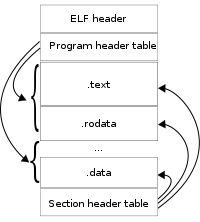
\includegraphics[width=0.5\textwidth]{elf}
	\caption{elf文件结构}
\end{figure}
\par 可执行的elf文件中,elfheader指定了程序的entry point,program header指定了代码段在文件中的偏移量。直接读取对应数据,将文件中的代码和数据段加载到内存0x100000处,再跳转至entry point执行即可。
\par 在加载和运行用户程序前,内核需要初始化串口,idt,中断,段寄存器,vga和键盘设备。其中大部分内容框架代码已实现,只需要补充idt的初始化。通过查阅相关资料,知键盘中断号是0x21,系统调用中断号是0x80,据此填写即可。需要注意系统调用的dpl为3。
\lstinputlisting[style=c]{idt.c}
\par 完成初始化后,就可以加载用户程序了。加载用户程序的过程与加载内核的过程基本相同,此处不再赘述。之后,内核通过iret指令进入用户空间,执行用户程序。

\subsection{中断服务和系统调用}
首先阅读实验代码中对中断处理的框架。各个中断服务程序将中断相关信息保存至栈中,然后统一调用asmDoIrq,保存现场并调用对应的irqHandle,通过TrapFrame的数据结构传递保存在通用寄存器内的参数。irqHandle再根据保存的中断号调用对应的中断处理函数。我们需要在此基础上实现对不同中断的特定处理程序。
\par 由于框架代码已给出了putChar函数,它可以将指定的字符从串口输出。由此可以封装自己的log函数,供调试使用。
\lstinputlisting[style=c]{log.c}

\subsubsection{键盘按键输入的处理}
由于填写好了键盘中断的idt,按下键盘的按键后最终会执行到函数KeyboardHandle。按键回显实现非常简单,直接对按键转换后的ascii码调用putChar即可。下面重点阐述键盘输入在vga上显示的处理方法。
\par 打印单个字符的方法已在指导文件中给出,可以将其封装为一个函数,方便后续使用:
\lstinputlisting[style=c]{printchar.c}

\par 将所有的按键分为以下4类:
\begin{itemize}
	\item 普通按键。这一类主要包含字母,数字和符号,处理方法也很简单,直接输出即可。
	\item 功能按键。这一类包含shift, control, capslock, tab等,这些按键可以不用显示。
	\item enter。需要注意光标的移动,要能够正确维护光标的位置,不需要输出字符。
	\item backspace。需要注意光标的移动,还要输出一个空格来覆盖原来可能存在的字符。而根据要求,backspace还只能删除自己输入的字符,因此还涉及输入缓冲区的维护(输入缓冲区相关内容将在最后一小节详细阐述)。
\end{itemize}
\par 根据上述特征,KeyboardHandle应该这样实现:
\lstinputlisting[style=c]{keyboard.c}

\subsubsection{打印字符串和printf的实现}
实现了键盘按键输入的vga显示后,打印字符串的功能就很容易实现了。只需要特殊处理换行符号,剩下的直接输出。光标维护的方法与上一小节完全相同,代码也高度相似,此处省略。
\par 函数printf的实现并不困难,只需要根据4种格式,调用对应的函数即可。需要注意计数必须准确。
\lstinputlisting[style=c]{printf.c}

\subsubsection{输入字符串的实现}
为实现输入的功能,必须维护一个输入缓冲区,键盘按键时将对应的字符加入缓冲区,系统调用输入字符串时将取出的字符(串)从缓冲区中删除。因此需要建立数据结构InputBuf。
\lstinputlisting[style=c]{inputbuf.c}
\par 但仅仅有上述插入删除功能还不够,还需要能够在缓冲区为空且执行getChar或getStr的系统调用时阻塞用户进程,直到用户在终端中输入字符(串)。阻塞解除的条件是输入回车,因此可以先开中断再执行hlt指令,直到检测到用户输入回车,再关中断,执行接下来的流程。由此,可以这样实现从缓冲区中获取字符(串)的方法:
\lstinputlisting[style=c]{retrive.c}
\par 实现这样的数据结构之后,只需要简单地调用它的方法就可以实现getChar和getStr了。键盘输入时维护缓冲区的相关代码在本节第1小节。

\section{实验结果}
kernel可以正确加载用户程序运行,并提供打印字符串,键盘输入并在串口和vga上回显,读取输入字符的中断服务程序。用户程序中的printf工作正常。
\begin{figure}[htbp]
	\centering
	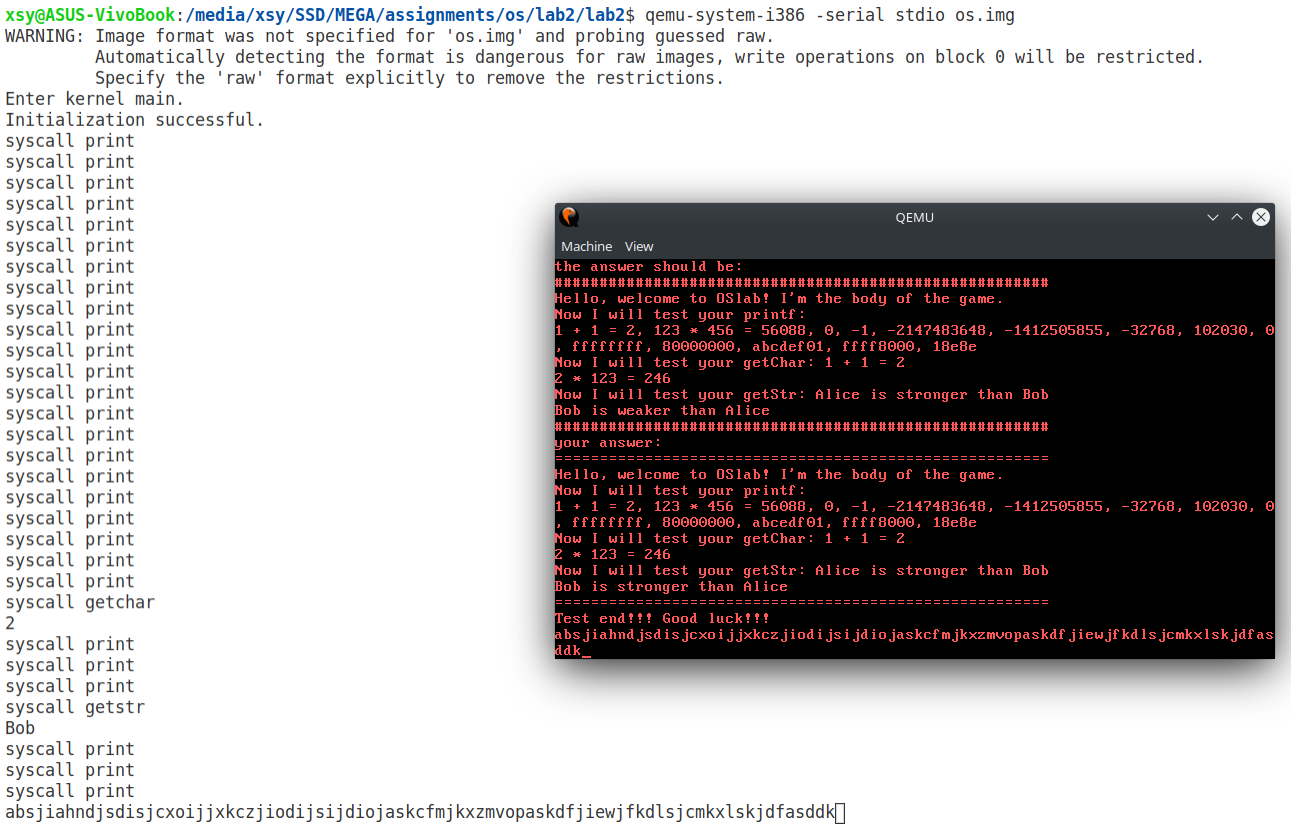
\includegraphics[width=\textwidth]{result}
	\caption{实验结果}
\end{figure}


\section{问题与思考}
\begin{enumerate}
	\item 一开始直接使用框架代码给出的makefile进行编译并执行,但发现报错"boot block too large",于是根据实验0的相关指导将命令改为objcopy -S -j .text -O binary bootloader.elf bootloader.bin,即可正确完成编译。
	\item 在命令行中运行qemu-system-i386 os.img,窗口显示"no bootable device"。通过询问助教,得知原因可能是gcc版本问题。安装gcc6并编译可成功运行。另外,一位学长(计网助教)给出的解决方案是加一个编译参数-fno-asynchronous-unwind-tables,经过尝试也可以成功。查询相关资料知,"This option determines whether unwind information is precise at an instruction boundary or at a call boundary. If -fno-asynchronous-unwind-tables is specified, the unwind table is precise at call boundaries only."新版本的gcc默认行为是"-fasynchronous-unwind-tables",而旧版的gcc默认"-fno-asynchronous-unwind-tables"。猜想unwind information的位置不同将影响加载过程,而qemu模拟的是老式的硬件,可能会产生不匹配。
	\item kernel按照-O1编译可以正常工作,但如果用-O2编译就会出现问题(getStr函数无法响应回车输入,一直保持阻塞状态)。根据以往经验,猜想可能是因为存在未初始化的变量,但仔细查找后并没有发现。有可能是因为kernel作为操作系统内核有特殊性,不能盲目开启优化。
\end{enumerate}

\section{建议}
\begin{enumerate}
	\item 框架代码修改建议:在框架代码中初始化gdt时,用户段的段描述符是将base设置为0x200000,而Makefile中-Ttext是0。因此,框架代码是想通过段基地址转换的偏移量访问用户代码和数据。但是,这样的想法和linux的实现方式相违背的。在linux中,用户段的base=0, limit=0xffffffff,即不使用段基地址转换。我一开始阅读框架代码,以为实现方式与linux相同,于是直接将-Ttext改为0x200000,没有仔细看gdt的初始化部分,导致后面运行出现问题,浪费了很多时间。而且,像我这样操作的同学还很多,可见这一想法是自然的,是框架代码的实现方式不佳。因此,我希望能进行如下修改:将app/Makefile中的-Ttext改为0x200000,在kernel/kernel/kvm.c中把用户代码和数据段描述符改为
	\lstinputlisting[style=c]{gdt.c}
	\item 修改Makefile:
	\begin{itemize}
		\item 不要使用-O2优化,可能会出现问题;
		\item 编译参数里添加-fno-asynchronous-unwind-tables。
	\end{itemize}
\end{enumerate}

\end{document}